\documentclass[aspectratio=1610]{beamer}

\usetheme{unnslides}
\usefonttheme{professionalfonts}

\usepackage[T2A]{fontenc}
\usepackage[utf8]{inputenc}
\inputencoding{utf8}
\usepackage[russian]{babel}
\usepackage{listings}
\usepackage{graphicx}
\usepackage{caption}
\usepackage{cmbright}
\usepackage{fontspec}
\usepackage{unicode-math}
\usepackage{amsfonts}
\usepackage{subfig}
\usepackage{tikz}

\captionsetup[subfigure]{labelformat=empty}
\captionsetup[figure]{labelformat=empty}

\setmainfont{CMU Sans Serif}
\setromanfont{CMU Sans Serif}
\setsansfont{CMU Sans Serif}

\setlength{\tabcolsep}{1pt}

\usepackage{polyglossia}
\setmainlanguage{russian}
%\setbeamertemplate{itemize item}{\color{black}$\blacktriangleright$}

\DeclareMathOperator*{\argmax}{arg\,max}
\DeclareMathOperator*{\argmin}{arg\,min}
\DeclareMathOperator{\sign}{sign}
\DeclareMathOperator{\re}{Re}

\graphicspath{ {../images/}{img/} }

%set pages numeration
\newcommand\numbered{\setbeamertemplate{footline}{%
  \vspace{-10em}
   \raisebox{5pt}{\makebox[\paperwidth]{%
     \hfill\makebox[10pt]{%
       \usebeamerfont{footline}\usebeamercolor[fg]{footline}
       \insertframenumber}}}}}
\newcommand\unnumbered{\setbeamertemplate{footline}{}}

\title{Параллельный алгоритм для получения равномерного приближения решений множества задач глобальной оптимизации с нелинейными ограничениями}
\author{\underline{\textbf{В.В.~Соврасов}} \and \textbf{К.А.~Баркалов}}
\institute{Нижегородский государственный университет им. Н.И. Лобачевского}
\date{}

\begin{document}
\numbered
{
\unnumbered
\begin{frame}[noframenumbering,plain]
\titlepage
\end{frame}
}

\begin{frame}
  \frametitle{Постановка задачи}
  \begin{columns}
    \begin{column}{0.5\textwidth}
      \begin{displaymath}
        \begin{array}{cr}\\
          \varphi(y^*)=\min\{\varphi(y):y\in D\}, \\
          D=\{y\in \mathbb{R}^N:a_i\leq y_i\leq{b_i}, 1\leq{i}\leq{N}\}
        \end{array}
      \end{displaymath}
      \(\varphi(y)\) -- многоэкстремальная функция, удовлятворяющая условию Липшица:
      \begin{displaymath}
        |\varphi(y_1)-\varphi(y_2)|\leq L\Vert y_1-y_2\Vert,y_1,y_2\in D,
      \end{displaymath}
      где \(L>0\) константа Липшица и \(||\cdot||\) обозначает \(l_2\) норму в пространстве \(\mathbb{R}^N\).
    \end{column}
    \begin{column}{0.5\textwidth}
      \centerline{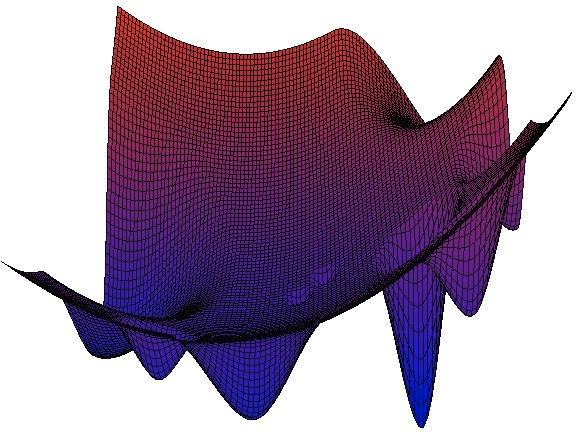
\includegraphics[width=0.9\textwidth]{img/gkls.png}}
    \end{column}
  \end{columns}
\end{frame}

\begin{frame}
  \frametitle{Заключение}
    \begin{itemize}
      \item
    \end{itemize}
\end{frame}
{
\unnumbered
\begin{frame}{{}}
  \frametitle{Q\&A}
  \begin{center}
    \Large{Contacts:}
\vspace{0.5cm}

    sovrasov.vlad@gmail.com

    https://github.com/sovrasov
  \end{center}
\end{frame}
}
\end{document}
